\documentclass{article}

\usepackage[a4paper,total={18cm,25cm}]{geometry}
\usepackage[spanish]{babel}

\usepackage{hyperref}
\usepackage{graphicx}
\usepackage{makeidx}

\graphicspath{{components/}}

\title{Animals clasifier}
\author{Alejandro García Villalba, Sofía Díaz Fernandez, Óscar Herrero Gordaliza}

\begin{document}
    \maketitle
    \begin{figure}
        \centering
        
\includegraphics[width=8cm]{politecnica_logo.png}
        
\includegraphics[width=8cm]{etsisi_logo.png}       
    \end{figure}

    \newpage

    \tableofcontents
        \section{Contexto}
        \section{Arquitectura}
        \section{resultados}

    \newpage

    \section{Contexto}

    Animals clasifier es una IA creada para distinguir distintas especies de animales, entre ellos están: Perros,caballos, elenfantes, mariposas, 
    gallinas, gatos,vacas, ovejas, arañas y ardillas.\newline
    
    \begin{figure}[h]
        \centering
        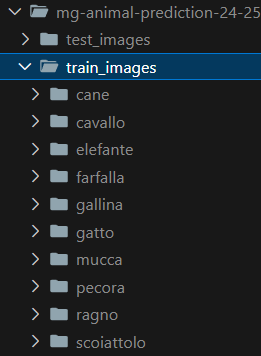
\includegraphics{dataset_images.png}
        \caption{Imágen del conjunto de imágenes¡}
    \end{figure}

    Para entrenar esta neurona hemos escogido un dataset perteneciente a un concurso de kaggel llamado \href{https://www.kaggle.com/competitions/mg-animal-prediction-24-25}{mg-animal-prediction-24-25}. 
    Este dataset ha sido creado como reto educativo para la asignatura de métodos generativos, como introducción al entrenamiento de redes de neuronas 
    densas y convolucionales.Cabe añadir, con motivo de aprendizaje, este documento se redacta en latex como primer contacto para proyectos posteriores,
    por su versatilidad a la hora de diseñar la estructura de la documentación de manera mas flexible.
    
    \begin{figure}[h]
        
\includegraphics[width=10cm]{Kaggle_logo.png}
        \centering
        \caption{\href{https://www.kaggle.com}{Imágen logotipo kaggle}}
    \end{figure}

    \newpage

    \section{Arquitectura}

\end{document}